\documentclass[a4]{article}

\usepackage[T1]{fontenc}
\usepackage[icelandic]{babel}
\usepackage{amsmath}
\usepackage{graphicx}
\usepackage{sidecap}
\usepackage[utf8]{inputenc}
\usepackage[left=1in,top=1in,right=1in,bottom=1in,nohead]{geometry}
\usepackage[framed,numbered,autolinebreaks,useliterate]{../mcode}
\usepackage{amsfonts}
\usepackage{epstopdf}

\lstset{language=MATLAB}
\title{Töluleg Greining\\ Heimaverkefni 3}
\date{\today{}}
\author{ 
  Bjarki Geir Benediktsson,\and
  Haukur Óskar Þorgeirsson,\and
  Matthías Páll Gissurarson \and
  Kennari: Máni Maríus Viðarsson
  }



\begin{document}
\begin{flushright}
  Bjarki Geir Benediktsson,\\
  Haukur Óskar Þorgeirsson,\\
  Matthías Páll Gissurarson\\
\end{flushright}

\begin{center}
 \textsc{ \LARGE Töluleg Greining\\
  Heimaverkefni 3\\
  \today{}
  }
  \end{center}
\vfill

\maketitle
\section{Forsagnar- og Leiðréttingaraðferð}
\subsection{}
\lstinputlisting[inputencoding=utf8]{adams_pc5.m}
\subsection{}
\lstinputlisting[inputencoding=utf8]{adams_pc5plot.m}
\lstinputlisting[inputencoding=utf8]{adams_pc5test.m}
Sjá myndir \ref{fig:adamspc5plot} og \ref{fig:adamspc5err}.
\begin{figure}[]
  \begin{center}
    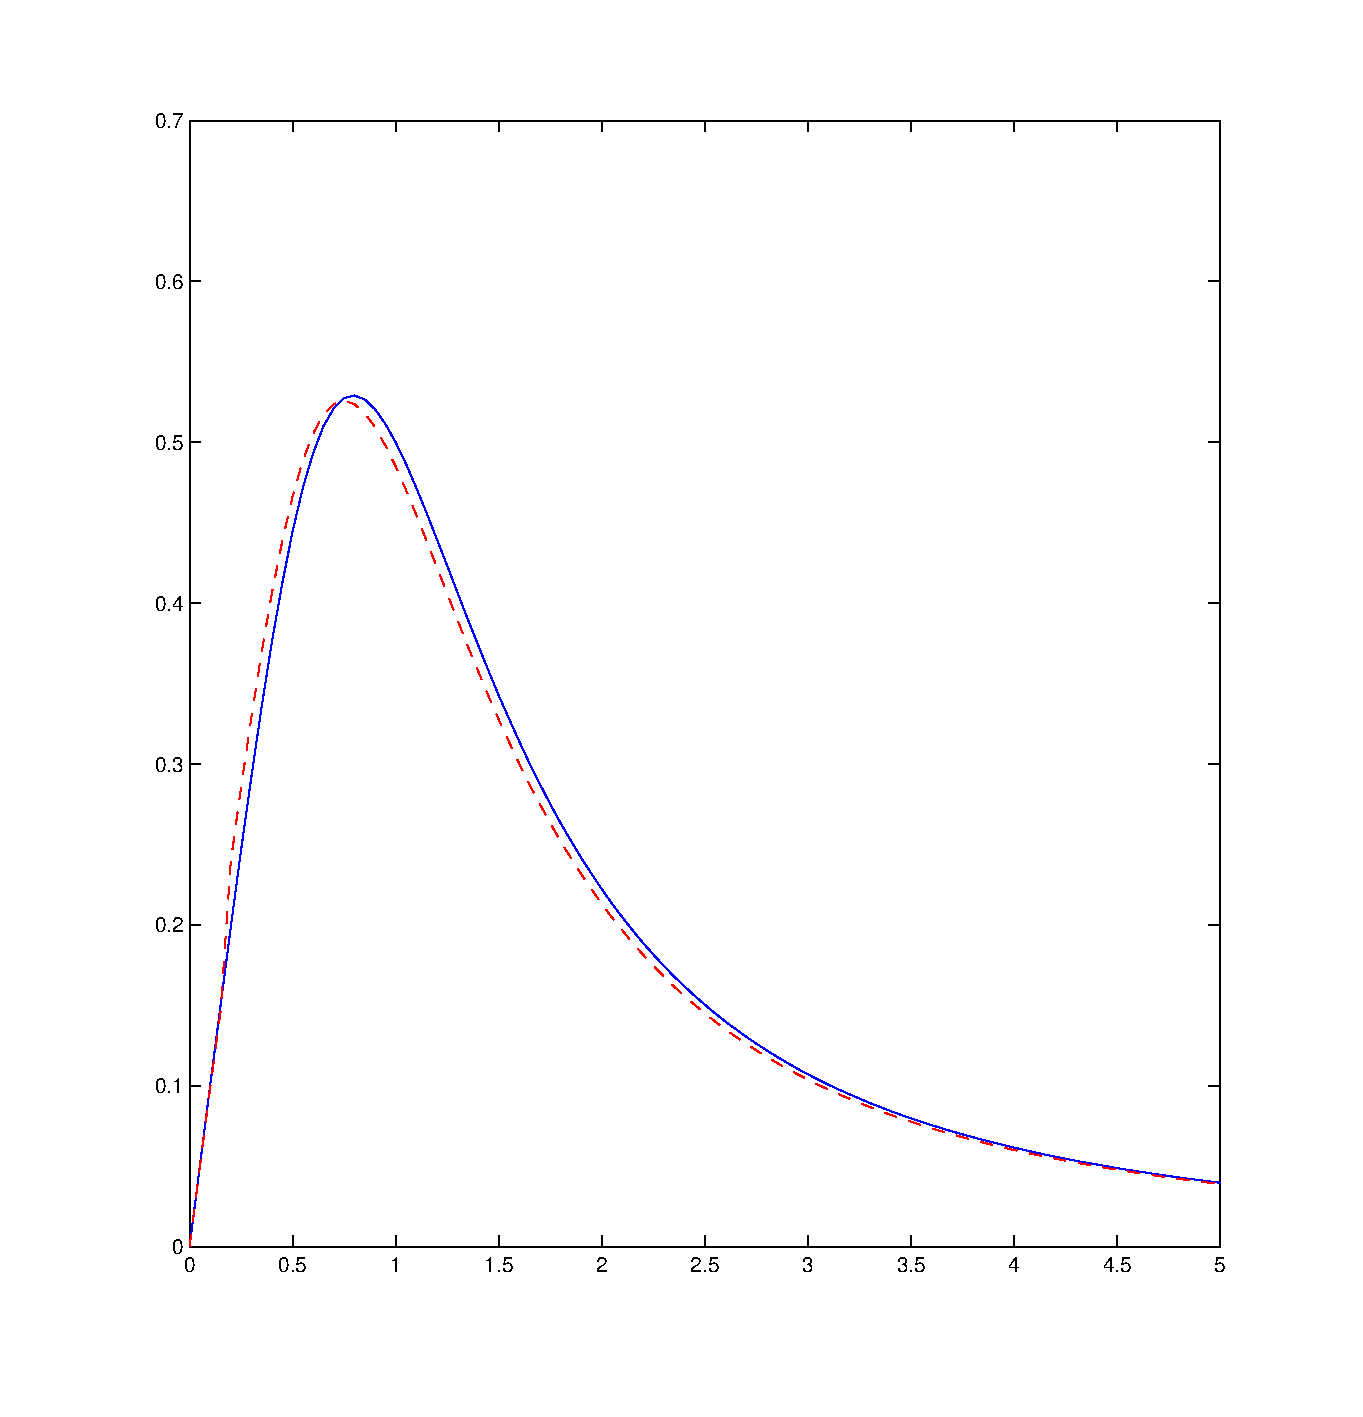
\includegraphics[scale=0.5]{adamspc5plot.eps}
  \end{center}
  \caption{Fallið sem prófa átti í 1, auk nálgun þess með adams\_pc5 sem rautt brotastrik}
  \label{fig:adamspc5plot}
\end{figure}
\begin{figure}[h]
  \begin{center}
    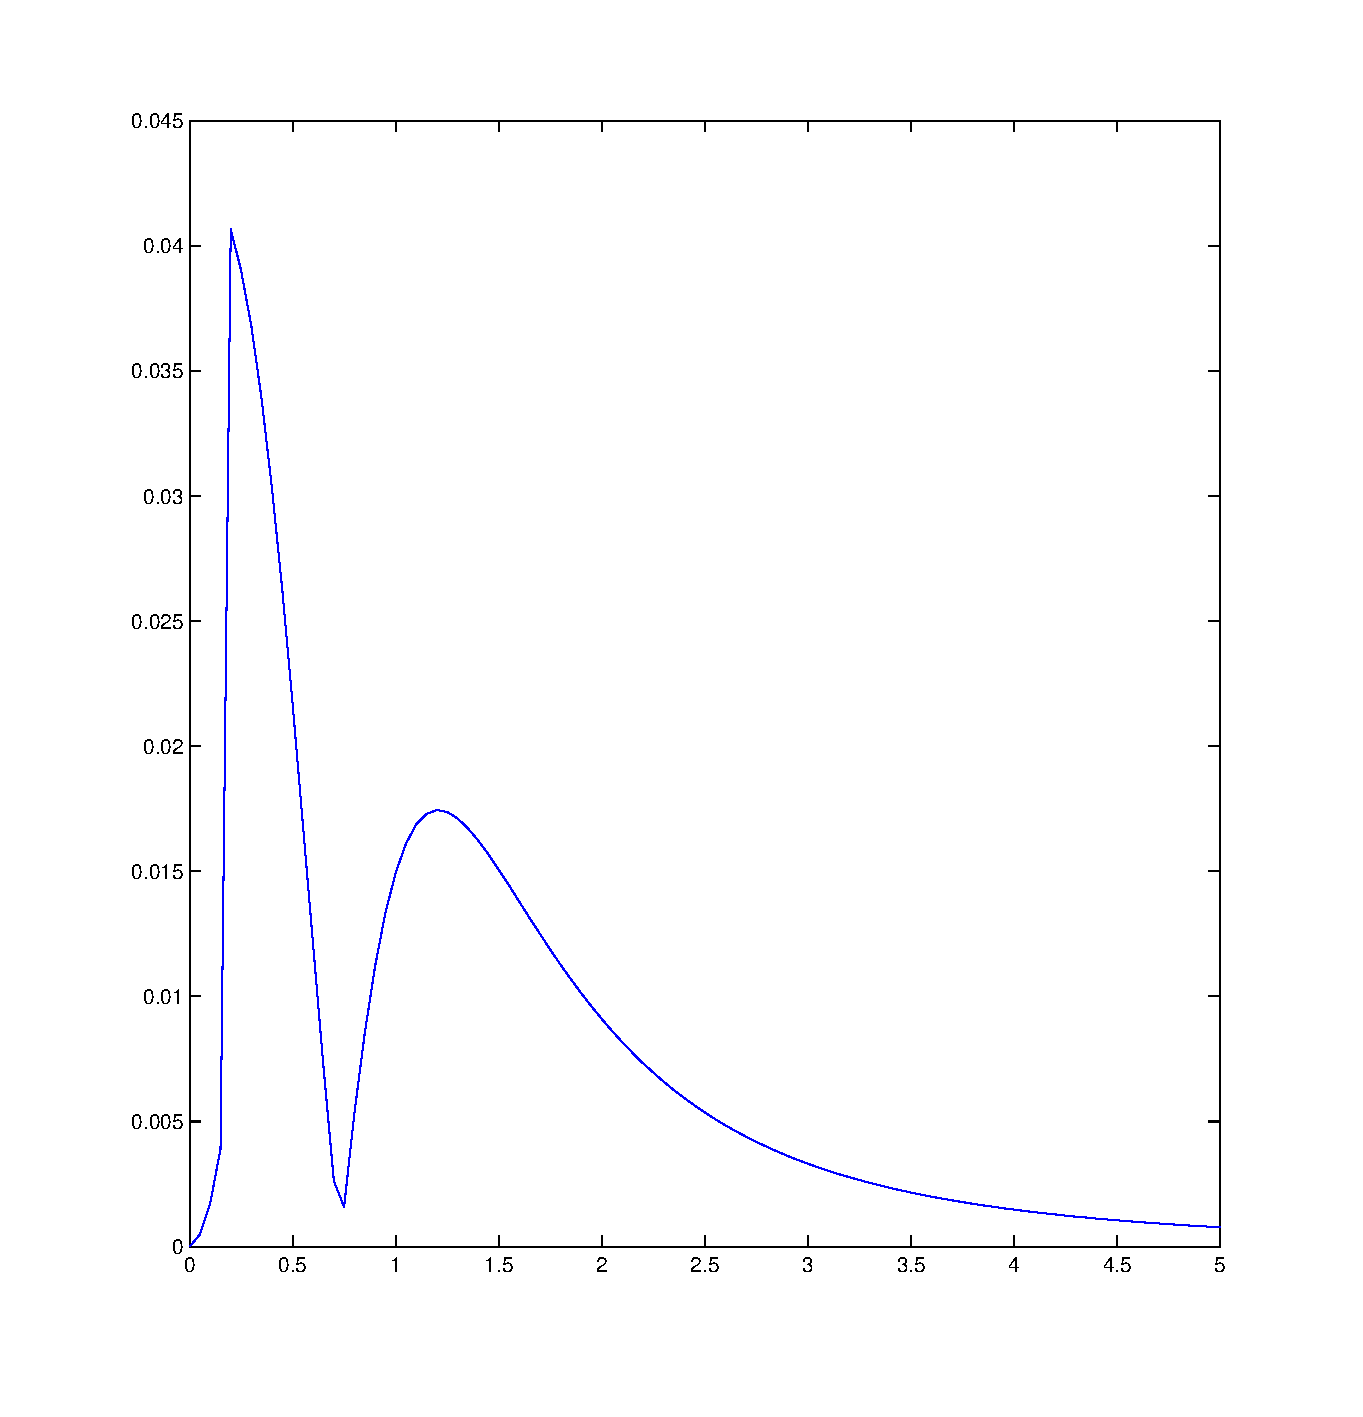
\includegraphics[scale=0.5]{adamspc5err.eps}
  \end{center}
  \caption{Skekkjan milli nálgunar þess með adams\_pc5 og fallsins sem prófa átti í 1 sem fall af t}
  \label{fig:adamspc5err}
\end{figure}
\subsection{}
til þess að fá heildarskekkju minni en $10^{-4}$ þurfti $h=\frac{1}{50000}=2*10^{-5}$

\subsection{Tímamælingar}
\lstinputlisting[inputencoding=utf8]{Timetake.m}
%athuga hvort það þurfi að breyta gildunum í take Taketime og uppfæra þá þessi gildi
Keyrsla á þessu forriti gaf eftirfarandi niðurstöður\\
\begin{tabular}{|c|c|}
\hline
fall		&meðatími \\\hline
adams\_pc5	&0,0082\\\hline
rkf45		&0,0024\\\hline
rkv56		&0,0027\\\hline
\end{tabular}


\section{Einfaldur pendúll}
Við fáum að þar sem $$\theta''(t) + \frac{g/l} \cdot \sin{ \theta(t)} \Leftrightarrow \theta''(t) = -\frac{g}{l} \cdot \sin{\theta(t)}$$
  þá má rita $$\left\{ \begin{array}{l} y(t) = \theta'(t) \\ y'(t) = \theta''(t) = - \frac{g}{l} \cdot \sin{\theta(t)} \end{array} \right.$$
Notum þetta til að skilgreina eftirfarandi fall:
\lstinputlisting[inputencoding=utf8]{pendulODE.m}
\lstinputlisting[inputencoding=utf8]{pendulApprox.m}

Við notuðum síðan þetta til að teikna hreyfimyndir, en það var gert með
\lstinputlisting[inputencoding=utf8]{pendull.m}

Með því að prófa nokkur gildi og horfa á útkomuna, þá komumst við að því að upphafhornið
$\theta_0 = 0.42$ gaf okkur frekar góða nálgun að 3 umferð, en eftir það fóru lausnirnar að greinast í sundur.

Til þess að svo gera hreyfimyndina þar sem útslagið er stórt var notaður eftirfarandi forritsbútur:
\lstinputlisting[inputencoding=utf8]{hr2.m}

\section{Róla}
  Við athugum að jafnan er eins og í 2, nema nú er lengdin auk þess fall af t. því fæst jöfnuhneppið
  $$\left\{ \begin{array}{l} y(t) = \theta'(t) \\ y'(t) = \theta''(t) = - \frac{g}{s(t)} \cdot \sin{\theta(t)} \end{array} \right.$$ 
  en $$s(t) = l + a*(cos \omega t + \varphi),$$
  þar sem l er lengdin, a er ústlagið, $\omega$ er horntíðnin og $\varphi$ er fasahliðrunin.
  
  Eftirfarandi tvö föll voru gerð til þess að nota með adams\_pc5, en fyrra er fyrir rólu sem er að hægja á sér og seinna er fyrir rólu sem er að hámarka útslagið. Munurinn liggur í mismunandi fasahliðrunum.
  \lstinputlisting[inputencoding=utf8]{roluODEmin.m}
  \lstinputlisting[inputencoding=utf8]{roluODEmax.m}

  Til þess svo að teikna meðfylgjandi myndbönd var notast við eftirfarandi skrá og pendull.m úr fyrri lið.
  \lstinputlisting[inputencoding=utf8]{hr3.m}.
  
  Útslagið örvaðist mest þegar $\omega = 1/T$ eins og gefið var í 3 og fasahornið var $\pi$,
  en ef $\varphi = 0$, þá hægði maður á rólunni. Munurinn liggur í hvenær maður styttir og lengir bandið, en ef fasahornið er 0, þá er mesta lengingin í miðjunni og minnst í endapunktunum,
  en öfugt er farið þegar hægt er á rólunni. Útskýringin á þessu er að maður er að nýta sér  hröðunina sem þyngdarkrafturinn veitir, en með því að vera að lengja á meðan maður dettur er maður í raun að detta meira beint niður.
  %%LAGA! SENNILEGA EKKI RÉTT
\section{Kúlupendúll}
 Jöfnuhneppið er einfaldlega það sama og gefið er í liðnum, en það má sjá í 
\lstinputlisting[inputencoding=utf8]{kulupendulODE.m}

 Eftirfarandi forritsbútur var notaður til að búa til myndbandið.
\lstinputlisting[inputencoding=utf8]{hr4.m}
 Það var gert með hjálp eftirfarandi falls, sem er pendúlsteiknifallið breytt til þess að ráða við þrívídd.
\lstinputlisting[inputencoding=utf8]{pendull3d.m}

\section{Lorenz}
\vspace{20 mm}
Að skýrsluni unnu :
\hspace{0.5cm} \makebox[1.5in]{\hrulefill}
\hspace{0.5cm} \makebox[1.5in]{\hrulefill}
\hspace{0.5cm} \makebox[1.5in]{\hrulefill}
\end{document}
